\section{Propuesta}
\label{sec:propuesta}

La propuesta consiste en un sistema modular de autenticación biométrica facial con almacenamiento cifrado, detección de \textit{liveness} y un módulo accesorio de detección de anomalías financieras. Toda la funcionalidad se expone mediante una CLI orquestada en \texttt{main.py}, organizada en tres familias de comandos: gestión de usuarios, evaluación/calibración y control financiero.

\subsection{Arquitectura General}
\label{subsec:arquitectura}

El código se organiza en una estructura modular bajo \texttt{src/}: \texttt{data/} (carga y validación de datos faciales y financieros), \texttt{features/} (preprocesamiento CLAHE y MTCNN), \texttt{models/} (\textit{embedders}, \textit{liveness} y detección de anomalías), \texttt{evaluation/} (métricas, ROC, calibración) y \texttt{utils/} (criptografía y soporte). La configuración del sistema reside en \texttt{config/config.yaml}, lo que permite ajustar umbrales y rutas sin tocar el código.

\subsection{Pipeline de Verificación}
\label{subsec:pipeline}

El flujo de \textit{login} se compone de las siguientes etapas:

\begin{enumerate}[leftmargin=*]
    \item \textbf{Detección y alineamiento (MTCNN):} se localiza el rostro y se alinea afinmente a partir de cinco puntos de referencia.
    \item \textbf{Liveness gate (DenseNet201):} se evalúa la imagen en crudo; si la puntuación es inferior al umbral calibrado, se rechaza la solicitud sin invocar al \textit{embedder}.
    \item \textbf{Normalización fotométrica (CLAHE):} sólo si supera el \textit{liveness}, la imagen alineada se ecualiza para reducir variabilidad por iluminación.
    \item \textbf{Embedding (ArcFace o FaceNet):} se genera un vector L2-normalizado.
    \item \textbf{Comparación coseno:} se compara con la plantilla descifrada del usuario reclamado y se decide aceptar/rechazar según el umbral de similitud.
    \item \textbf{Control de intentos:} en caso de rechazo se incrementa un contador por usuario que activa un bloqueo temporal tras N fallos consecutivos.
\end{enumerate}

\subsection{Esquema de Seguridad}
\label{subsec:seguridad}

La protección de las plantillas se implementa en \texttt{src/utils/} y combina tres mecanismos:

\begin{itemize}
    \item \textbf{Confidencialidad:} cada \textit{embedding} se serializa y se cifra con Fernet (AES-128-CBC + PKCS7) \cite{fernet}.
    \item \textbf{Derivación de clave:} la clave Fernet se obtiene en cada arranque mediante PBKDF2-HMAC-SHA256 con 310.000 iteraciones y \textit{salt} aleatorio persistido, conforme a NIST SP 800-132 \cite{nist800132}.
    \item \textbf{Integridad:} junto al ciphertext se almacena un HMAC-SHA256 del \textit{embedding} en plano; cualquier manipulación del fichero de base de datos invalida la verificación y aborta el \textit{login}.
\end{itemize}

\subsection{Calibración y Evaluación}
\label{subsec:calibracion}

El subcomando \texttt{evaluate} calcula EER, ROC-AUC, F1 y TAR@FAR sobre un fichero \texttt{pairs.csv} con pares etiquetados; el subcomando \texttt{benchmark} compara latencia, rendimiento y separación coseno entre \textit{backends}; y el subcomando \texttt{tune} barre el espacio de umbrales de similitud y de \textit{liveness} y actualiza \texttt{config.yaml} con el punto de operación óptimo. Las salidas gráficas (curvas ROC, distribución de \textit{scores}, comparativas DET y mapa de barrido de umbrales) se persisten en \texttt{doc/evaluation/} para su inclusión en la memoria.

\subsection{Resultados Experimentales}
\label{subsec:resultados}

La evaluación del detector de \textit{liveness} se ha realizado sobre la partición de test del dataset Kaggle \textit{real-vs-fake-anti-spoofing-video-classification}, extrayendo tres \textit{frames} por vídeo en los segundos 3, 5 y 7 (conjunto disjunto del usado en entrenamiento). La Figura~\ref{fig:samples_live_spoof} muestra un mosaico representativo de muestras correctamente clasificadas en ambas clases, donde se aprecia visualmente la diferencia que el modelo aprende a discriminar.

\begin{figure}[tbp]
    \centering
    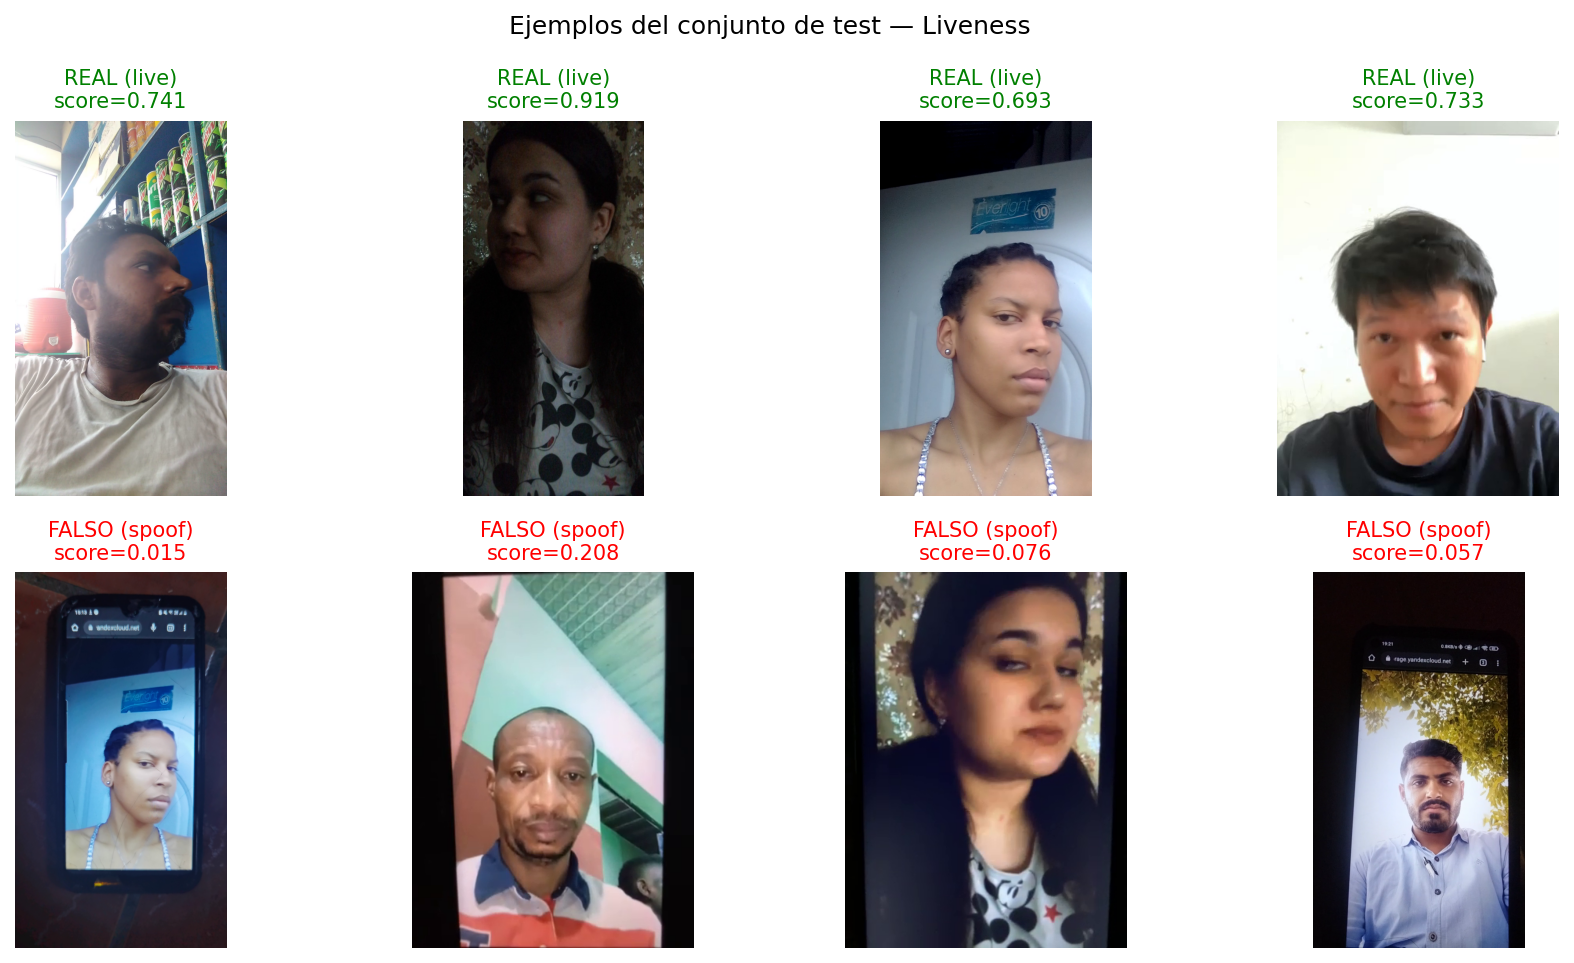
\includegraphics[width=0.85\textwidth]{evaluation/samples_live_vs_spoof.png}
    \caption{Ejemplos del conjunto de test del detector de \textit{liveness}: fila superior muestras reales (\textit{live}) y fila inferior ataques de presentación (\textit{spoof}). Se indica el \textit{score} de probabilidad de ser real predicho por el modelo.}
    \label{fig:samples_live_spoof}
\end{figure}

\begin{figure}[tbp]
    \centering
    \begin{subfigure}[tbp]{0.45\textwidth}
        \centering
        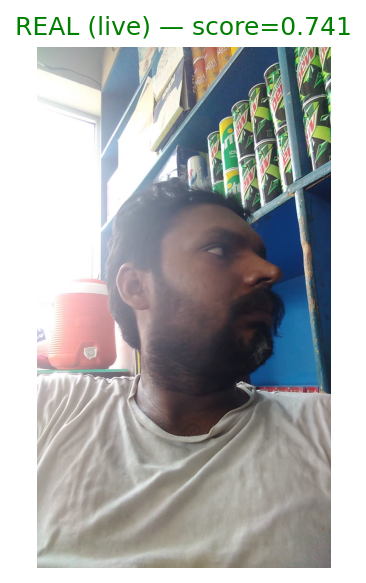
\includegraphics[width=\linewidth]{evaluation/sample_live.png}
        \caption{Muestra real (\textit{live}).}
        \label{fig:sample_live}
    \end{subfigure}
    \hfill
    \begin{subfigure}[tbp]{0.45\textwidth}
        \centering
        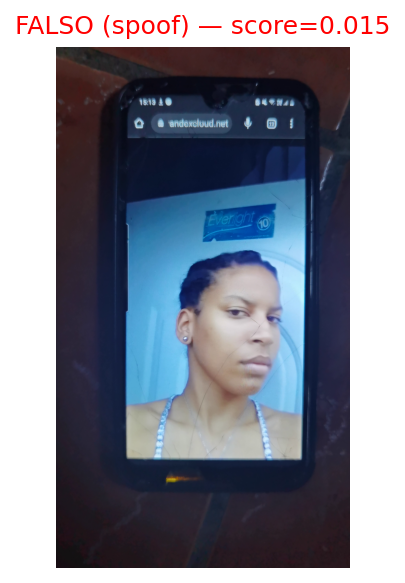
\includegraphics[width=\linewidth]{evaluation/sample_spoof.png}
        \caption{Muestra falsa (\textit{spoof}).}
        \label{fig:sample_spoof}
    \end{subfigure}
    \caption{Comparación directa de un \textit{frame} etiquetado como verdadero (izquierda) frente a uno etiquetado como falso (derecha) con su \textit{score} de \textit{liveness} asociado.}
    \label{fig:sample_compare}
\end{figure}

La Figura~\ref{fig:roc_liveness} presenta la curva ROC del detector y la Figura~\ref{fig:score_dist_liveness} la distribución de \textit{scores} para ambas clases, lo que permite observar la separabilidad alcanzada y justificar la elección del umbral de operación. La matriz de confusión resultante (Figura~\ref{fig:confusion_liveness}) resume los aciertos y errores de clasificación, ofreciendo una lectura directa de los falsos aceptos y falsos rechazos del sistema.

\begin{figure}[tbp]
    \centering
    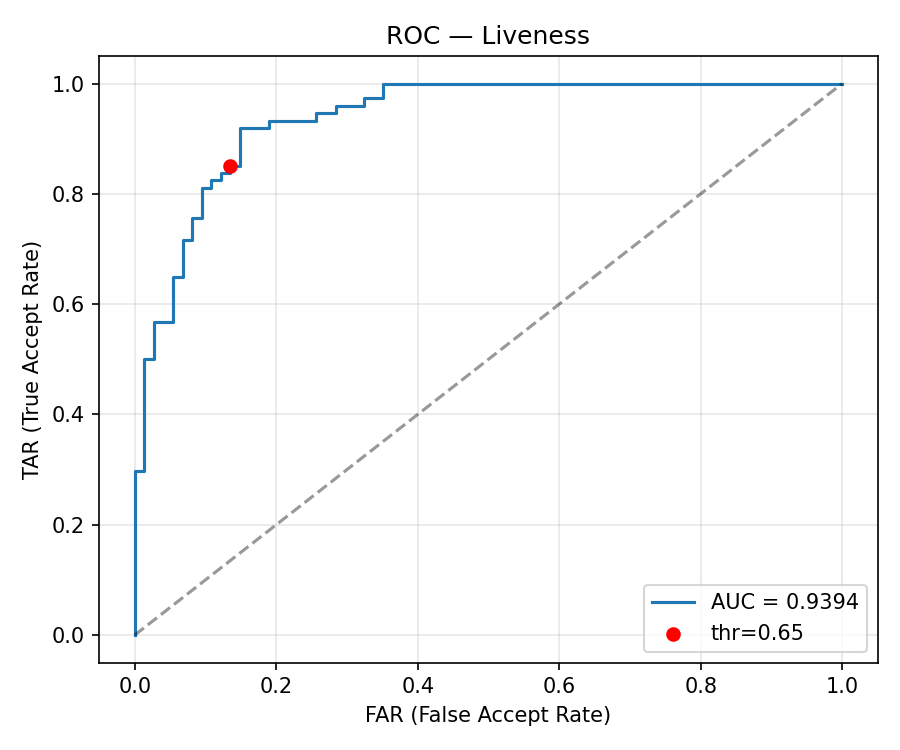
\includegraphics[width=0.7\textwidth]{evaluation/roc_liveness.png}
    \caption{Curva ROC del detector de \textit{liveness} sobre el conjunto de test. Se marca en rojo el punto de operación correspondiente al umbral configurado.}
    \label{fig:roc_liveness}
\end{figure}

\begin{figure}[tbp]
    \centering
    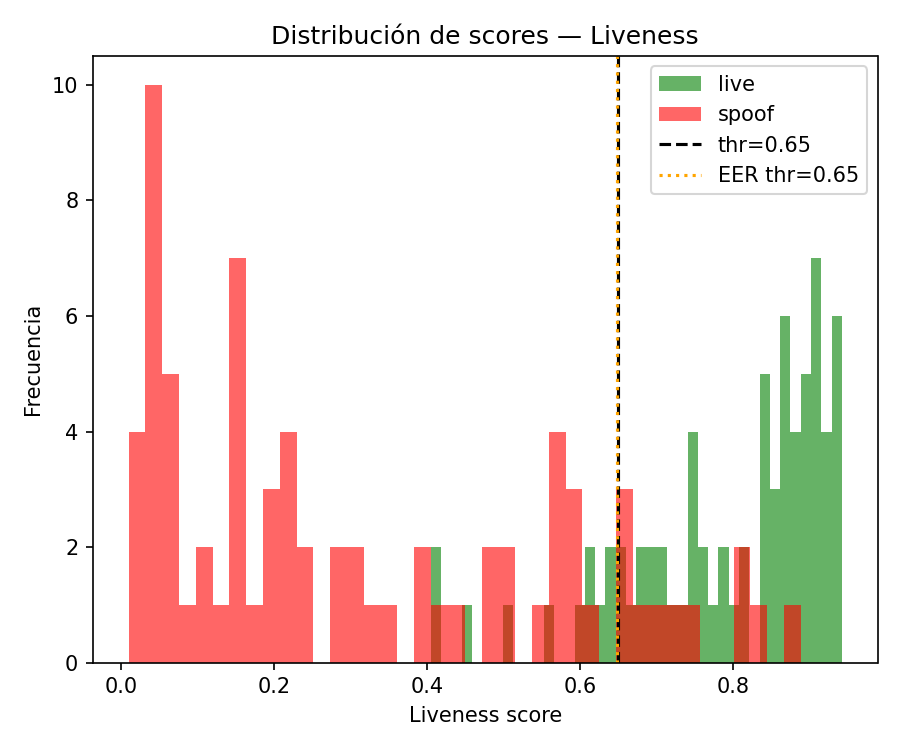
\includegraphics[width=0.7\textwidth]{evaluation/score_dist_liveness.png}
    \caption{Distribución de \textit{scores} de \textit{liveness} para muestras reales (verde) y de ataque (rojo), con el umbral actual y el umbral correspondiente al \textit{Equal Error Rate}.}
    \label{fig:score_dist_liveness}
\end{figure}

\begin{figure}[tbp]
    \centering
    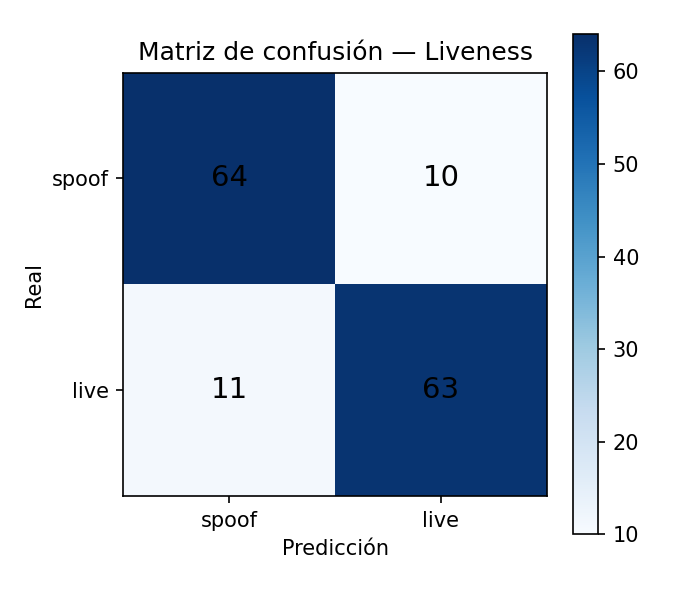
\includegraphics[width=0.55\textwidth]{evaluation/confusion_liveness.png}
    \caption{Matriz de confusión del detector de \textit{liveness} sobre la partición de test del dataset.}
    \label{fig:confusion_liveness}
\end{figure}

\subsection{Módulo Financiero}
\label{subsec:finanzas}

El comando \texttt{finance-add} valida cada nueva transacción mediante un detector híbrido: la regla de las 3-Sigmas filtra anomalías univariantes por categoría, y un \textit{Isolation Forest} \cite{liu2008isolation} captura combinaciones inusuales de \texttt{Cantidad}, \texttt{Área}, \texttt{Tipo}, \texttt{Mes} y \texttt{Día de la semana}. El modelo se reentrena tras cada confirmación, lo que aporta una adaptación continua al perfil del usuario sin requerir etiquetas.
